\documentclass[a4paper,12pt]{article}
\usepackage{../../../mypackages}
\usepackage{../../../macros}


\usepackage{pgfplots}
    \pgfplotsset{
    compat=1.11,
  }

\setlength{\parindent}{0pt}

\begin{document}

\title{Chapitre 2 - Les suites}
\author{N. Bancel}

\maketitle

\def\WITH_CORRECTION{YES}

\section*{Qu'est ce qu'une suite ?}

\begin{tcolorbox}[colback=green!10!white, colframe=green!75!black, title=Définition : xxx]
  Une suite numérique est une \trou{\textcolor{blue}{fonction}}{\ndots[10]} qui, à tout entier naturel $n$ (n = 0, 1, 2) associe un nombre réel noté $U(n)$ ou $U_n$.
  On parle du \trou{\textcolor{blue}{terme}}{\ndots[10]} de \trou{\textcolor{blue}{rang / d'indice $n$}}{\ndots[10]} de la suite.  Une suite est une liste ordonnée d'élements
\trou{
  \begin{figure}[H]
    \centering
    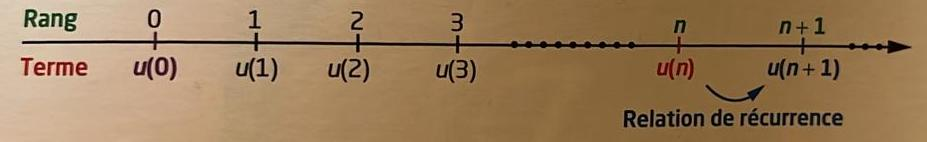
\includegraphics[width=0.9\linewidth]{schema_suites.jpeg}
    \caption{\label{} Suite}
  \end{figure}
}{\vspace{2em}}
\end{tcolorbox}

\textbf{Exemples} \par
\vspace{0.5em}
$u = \left\{15, -3, 7, 8, 97, ...\right\}$ est une suite. \par 
En faisant commencer l'indice de la suite à 0, le terme d'indice 4, noté $u(4)$ est égal à \trou{\textcolor{blue}{8}}{\ndots[3]} \par 
\trou{\[
u(4) = 8
\]}{\vspace{2em}}

\vspace{1em}

Dans certains cas on comptera les positions à partir de 0, dans d’autres à partir de 1 (l’énoncé dira quelle convention utiliser). \par
\vspace{1em}
Par exemple dans la suite $u$ ci-dessus :
\begin{itemize}[noitemsep]
  \item $u(2)= \trou{-3}{\ndots[4]}$ si on compte les positions à partir de 1,
  \item $u(2)= \trou{7}{\ndots[4]}$ si on compte les positions à partir de 0.
\end{itemize}

Si l’énoncé dit "pour tout entier naturel $n$" ou "pour $n \in \mathbb{N}$" , cela voudra dire que l’on compte à partir de 0.
De façon générale, on peut commencer notre suite à n’importe quel rang $n \geq 0$.

\subsection*{Exemples}

Soit $v$ la suite des nombres impairs. Donner $v(5)$ en supposant que les indices débutent à 0. \par
\vspace{1em}
\trou{
  Réponse: $v = \{1;3;5;7;9;11;...\}$, d’où $v(5) = 11$.
}
{\vspace{2em}}


\begin{tcolorbox}[colback=blue!10!white, colframe=blue!75!black, title=Exercices]
  Exercices 1, 3, 5, 6
\end{tcolorbox}

\section*{Représentation graphique d'une suite}
\vspace{1em}

La représentation graphique d’une suite $u$ sera un nuage de points. Ces points auront pour coordonnées $(n ; U_n)$.
En reprenant l’exemple de la suite u des multiples de 2, la représentation graphique de u est :

\trou{
  \begin{figure}[H]
    \centering
    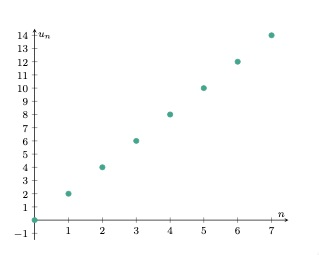
\includegraphics[width=0.5\linewidth]{representation_graphique.jpg}
    \caption{\label{} Représentation graphique}
  \end{figure}
}
{\vspace{7em}}

\section*{Suite définie comme une fonction}
\vspace{1em}

Plutôt que de donner chacun des termes d’une suite, on peut la définir à l’aide d’une formule. La première façon de définir une suite est à l’aide d’une \trou{\textbf{fonction du rang n}}{\ndots[20]}.
On dit que la suite est définie \trou{\textbf{de façon explicite / fonctionnelle.}}{\ndots[20]}

\begin{tcolorbox}[colback=blue!10!white, colframe=blue!75!black, title=Exercices]
  Soit $u$ la suite définie pour tout entier naturel $n$ par $u(n) = 2n - 3$. \par 
  On trouve chaque terme de la suite en remplaçant $n$ par 0,puis 1, 2, etc.
  Ainsi $u(10) = 2 \times 10 - 3 = 17$ et de façon plus générale $u = { \trou{\{-3 ; -1 ; 3; 3 ; ...\}}{\ndots[20]}}$. \par
  \vspace{1em}
  Représenter graphiquement la suite $U$
  \vspace{6em}
\end{tcolorbox}

C'est comme si on échantillonait une fonction (c'est-à-dire qu'on ne sélectionnait les valeurs que pour des valeurs de $x$ données (des nombres entiers))

\begin{figure}[H]
  \centering
  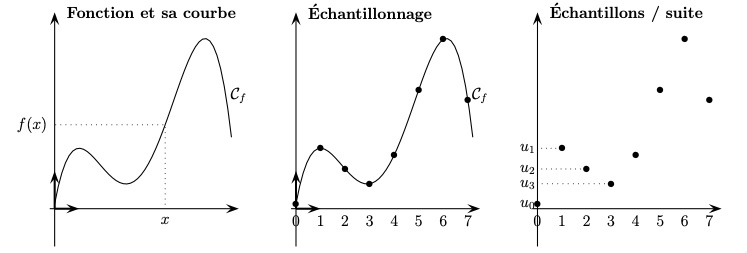
\includegraphics[width=0.8\linewidth]{echantillonage.jpg}
  \caption{\label{} Echantillonage}
\end{figure}

\begin{tcolorbox}[colback=blue!10!white, colframe=blue!75!black, title=Exercices]
  On considère la suite $U(n) = n^2$. Donner les 4 premiers termes de la suite en commençant à $n = 0$

  \trou{
    \[
    \left\{
      \begin{array}{ll}
            U(0) = 0 \\
            U(1) = 1^2 = 1 \\
            U(2) = 2^2 = 4 \\
            U(3) = 3^2 = 9 \\
        \end{array}
      \right.
    \]
  }{\vspace{5em}}

\end{tcolorbox}

\section*{Expression de $U_{N-1}$, $U_{N+1}$, $U_{2N}$, ...}

Si l’expression de $U_n$ est donnée, on peut donner celle de $U_{n+1}$ en remplaçant $n$ par $n + 1$ (en n'oubliant pas les parenthèses).
De même on peut donner l’expression de $U_{2n}$ en remplaçant $n$ par $2n$. \par
\vspace{1em}
\textcolor{blue}{Exemple} : Soit la suite $u$ définie pour tout entier naturel par
\[
  U_n = 7n + 5
\] \par

Donner l’expression de $U_{n+1}$ et de $U_{2n}$

\trou{\vspace{5em}}{\vspace{5em}}

\begin{tcolorbox}[colback=blue!10!white, colframe=blue!75!black, title=Exercices]
  Exercice N°17 page 123 et Question 2 de Exercice N°19
\end{tcolorbox}

\section*{Suite définie par récurrence}

\textbf{Préambule}
\vspace{1em}
Pour maîtriser la partie qui suit, il est nécessaire de comprendre que : 
\begin{itemize}[noitemsep]
    \item $u(n+1)$ est le terme après $u(n)$,
    \item $u(n)$ est le terme après $u(n-1)$,
    \item $u(n-1)$ est le terme après $u(n-2)$,
    \item etc.
\end{itemize}

Et aussi que :
\begin{itemize}[noitemsep]
    \item si $u(n+1)$ est $u(4)$, alors $u(n)$ est $u(3)$,
    \item si $u(n+1)$ est $u(12)$, alors $u(n)$ est $u(11)$,
    \item si $u(n)$ est $u(10)$, alors $u(n-1)$ est $u(9)$.
\end{itemize}


La seconde façon de définir une suite est par récurrence. Dans ce cas, pour calculer la valeur d’un terme de la suite, on a besoin d’un ou plusieurs termes précédents. Ainsi, on aura par exemple une formule du type :
\[
u_{n+1} = \ldots u_n \ldots
\]
ou
\[
u_n = \ldots u_{n-1} \ldots
\]

\begin{tcolorbox}[colback=blue!10!white, colframe=blue!75!black, title=Exercices]

  Soit la suite définie comme suit : 

  \[
    \left\{
      \begin{array}{ll}
            u(n+1) = 4 u(n) + 7 \\
            u(0) = -1 
        \end{array}
      \right.
    \]

  Calculer $u(1)$ et $u(2)$

  \trou{
  Pour calculer $u_1$
  $u(1) = 4u(0) + 7 = 4 \times (-1) + 7 = 3$

  Maintenant que l’on connaît $u_1$, on peut calculer $u_2$ : \\
  $u(2) = 4u(1) + 7 = 4 \times 3 + 7 = 19$

  }
  {\vspace{6em}}


  \textbf{Faire les exercices 66 et 68. Conjecturer le sens de variation }
\end{tcolorbox}


\end{document}
